\section{实验:安装直流电动机模型}\label{sec:10-11}

照图 \ref{fig:10-43} 把直流电动机模型安装起来。
安装时要尽量减小轴和轴架之间的摩擦,电刷跟换向器的接触不要太松也不要太紧。

画出用导线把电动机、电键、变阻器、电源串联起来的电路图,按照电路图连接好电路。
然后合上电键,注意观察线圈的转动方向。

\begin{wrapfigure}[9]{r}{7cm}
    \centering
    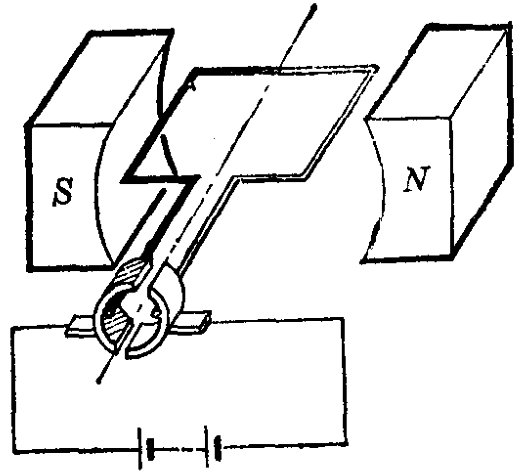
\includegraphics[width=6cm]{../pic/czwl2-ch10-44}
    \caption{}\label{fig:10-44}
\end{wrapfigure}

把电源两极对调一下,改变线圈中电流的方向,观察线圈转动的方向是否改变。
再把磁铁的两极对调一下,改变磁力线的方向,观察线圈转动的方向是否改变。

利用变阻器改变通过线圈的电流强度,观察转子转动的速度怎样随着变化。


\lianxi

(1) 图 \ref{fig:10-44} 是直流电动机的示意图。标出图上各部分的名称。

(2) 某个电动机模型不能运转了。发生故障的原因可能是磁铁没有磁性或者是换向器和电刷接触不良。
试说明你如何对这些地方进行检查。

(3) 一台电动机,额定电压是 220 伏特,电功率是 6 千瓦。它在正常工作的时候,电流强度是多大?

